\chapter{Mathematical Background}
\section{One-Shot Games}
\subsection{Prisoner's Dilemma}
The Prisoner's Dilemma is the canonical game of game theory, finding its use in models for everything from share prices to the relationship between lions and small birds. Essentially, in any situation where there is the possibility of cooperation, the Prisoner's Dilemma can be a useful model in understanding the situation to a first approximation.
\subsubsection{The Story}
The motivating story goes that two accomplices are caught at a crime scene, arrested and placed in seperate cells with no contact. The police give them each a choice: they can confess their crimes to the authorities (defect) or they can stay silent (cooperate).\\
They learn that if they both cooperate, they only get one year in prison. If they both defect, they both get two years. However, if one of them cooperates and the other defects, the cooperator gets 3 years and the defector gets out of jail immediately. As they are in seperate cells, they cannot communicate.\\
The smallest combined time in prison for the couple is if they both cooperate and take 1 year in jail each. But even if they could communicate and agree to the appealing option of both cooperating, it would still make sense to defect from the `contract' and defect. But just 1 year in jail is clearly better than 2. How should they work through this? As with most things in life, they should get mathematical.
\subsection{Making this Mathematical}
\subsubsection{Key Concepts}
This story has all the features of a game-theoretic game. Let's go through it, pick out the key elements and name them.\\
The four essential elements of a game have a useful acronym: \textit{PAPI} \cite{rasmusen}. This stands for:\\
the \textbf{P}layers of the game,\\
the \textbf{A}ctions available to each player,\\
the \textbf{P}ayoffs for each outcome\footnote{An \textit{outcome} defines an action for each player. It can be written $(C,C)$ for two players both playing the action $(C)$. Note, actions are usually represented as a single letter i.e. $(C)$ for cooperate and $(D)$ for defect. } and\\
the \textbf{I}nformation available to each player.\\

In our story, there are two players: Lou and Avery. The actions are cooperate with the partner in crime (i.e. stay quiet) or defect (i.e. confess and betray partner). The payoffs are given by the years in jail, $-x$ for $x$ years in jail. As they cannot communicate, there is no information available about the other player's choice prior to choosing.
\subsubsection{Representing games}
\subsubsection{Payoff Matrix}
A payoff matrix is a way of defining two-player simultaneous games completely i.e. it tells you about every element of \textit{PAPI}. The payoff matrix for the Prisoner's Dilemma given in the story would be:\\
\setlength{\extrarowheight}{2pt}
\begin{tabular}{cc|c|c|}
	& \multicolumn{1}{c}{} & \multicolumn{2}{c}{Avery}\\
	& \multicolumn{1}{c}{} & \multicolumn{1}{c}{$C$}  & \multicolumn{1}{c}{$D$} \\\cline{3-4}
	\multirow{2}*{Lou}  & $C$ & $(-1,-1)$ & $(-3,0)$ \\\cline{3-4}
	& $D$ & $(0,-3)$ & $(-2,-2)$ \\\cline{3-4}
\end{tabular}
\\
\\
The players, actions and payoffs are defined. Also there is no information available about the other player's action. So this matrix completely describes the game. Note that the the ordered pair $(x,y)$ in each matrix entry gives the payoffs for each outcome. $x$ gives the payoff for the horizontal player and $y$ gives the vertical player's. So outcome $(D,C)$ has payoff $(0,-3)$ meaning a payoff of $0$ for Lou for defecting and a payoff of $-3$ for Avery for cooperating.\\
The payoff matrix is an extremely useful representation, allowing concise, complete descriptions of games. Consider, for example:\\
\setlength{\extrarowheight}{2pt}
\begin{tabular}{cc|c|c|c|}
	& \multicolumn{1}{c}{} & \multicolumn{3}{c}{Avery} \\
	& \multicolumn{1}{c}{} & \multicolumn{1}{c}{$R$}  & \multicolumn{1}{c}{$P$}  & \multicolumn{1}{c}{$S$} \\\cline{3-5}
	& $R$ & $(0,0)$ & $(-1,1)$ & $(1,-1)$ \\ \cline{3-5}
	Lou  & $P$ & $(1,-1)$ & $(0,0)$ & $(-1,1)$ \\\cline{3-5}
	& $S$ & $(-1,1)$ & $(1,-1)$ & $(0,0)$ \\\cline{3-5}
\end{tabular}
\\
\\
This game might initially look foreign, but it is simply Rock, Paper, Scissors. You can create stories to motivate them but the payoff matrix completely defines all the relevant mathematical aspects of the game. This allows us to abstract from the messy details of the human world and find `solutions' to the game.
\subsubsection{Solution Concepts}
A \textit{strategy} is a set of rules for which actions to play at each point of the game. It can respond to the other player's actions.
\subsubsection{Strategies}
\paragraph{Socially Optimal Strategy}Lou is able to recognise the \textit{socially optimal strategy} as the option of both cooperate so that they get only 1 year each. This is the outcome that leads to the highest joint payoff for all players.
\paragraph{Nash Equilibrium} However, the outcome with both defecting is the Nash Equilibrium. This is an outcome in which, even if all players knew what the rest of the players actions were, none of them would choose to change their action as it would not improve their payoff. In this game, both players defecting is the unique Nash Equilibrium.
\paragraph{Dominant Strategy}The outcome of $(D, D)$ actually satisfies a stronger condition as the action defect is a \textit{dominant strategy} for both players. This means that no matter what action the opponent plays, the player can always increase their payoff by defecting. This is the way (defect, defect) `pulls' players in, despite it having a worse payoff for both players than cooperate cooperate. Game theory assumes that players are \textit{rational} (i.e. the payoffs we have described actually match their desires and they are aware of how the game works). So if Lou and Avery are rational, they will always end up both defecting, betraying each other and being rewarded with a longer jail term. So it goes.

\section{Repeated Games}
\subsubsection{Introduction}
The previous games are called \textit{one-shot games} meaning, after the first game is played, no further games are played. It happens once and never again, with no possible repurcussions that are not already described in the payoff matrix.\\

Unlike one-shot games, repeated games have players play multiple games against each other. This means that it is harder or even impossible to `solve' these games to find the best actions and equilibria. However, this makes them more interesting, allowing for complex dynamics. For example, the prisoner's dilemma no longer has a best strategy when repeated.
\subsubsection{Repeated Prisoner's Dilemma Tournament}
We can create a tournament of different strategies all playing several hundred games against each other. The winner is the strategy with the highest payoff overall. This numerical experiment was famously first done by Robert Axelrod\cite{axelrod} in the 1980s. In Axelrod's first tournament, the winner was `Tit for Tat', a strategy that always cooperates on the first round and then copies the opponents previous move forever after.\\
(
My simulation of Prisoner's Dilemma tournament.\\
Include Tit for Tat, Grim Trigger, Random, always cooperate, always defect, tit for two tats etc.\\
brief analysis of my results- graph of results
)

\subsubsection{Repeated Games with Evolution}
[Include replicator equations at some point here.]\\
Incorporating repetitions, allows the possibility of 'evolutionary' behaviour. For example, one can create simulations where higher payoffs are more likely to produce 'offspring' i.e. players that use the same strategy. For example, below is a simulation of strategies playing Rock, Paper Scissors defined by the payoff matrix as above.\\
(
My simulation of Rock, Paper, Scissors
)\\
The effect is a self-balancing system. If the strategy \textit{rock} becomes more populous, \textit{paper} will start to get higher payoffs on average. This in turn brings the population back towards $\frac{1}{3}$ for each strategy.\\
The same scenario works with the admitedlly less well-known game Rock, Paper, Scissors, Spock\cite{for game}\cite{for code}.\\
(
My simulation of Rock, Paper Scissors, Spock
)\\
However, now with the different rules we can have the extinction of strategies.
\section{Games on Graphs}
In real life, games are usually not isolated situations that happen as if in a laboratory. Instead, we take part in many at the same time with several different players. Sometimes the different games effect each other. To model this, we can use graphs.
\subsubsection{Graphs}
A graph $G=(V,E)$ is a set of vertices $V$ and a set of edges $E$ which are pairs of vertices. For now we will consider only undirected ($(u,v)\in E\iff(v,u)\in E$) graphs with no loops ($\nexists v\textnormal{ s.t. } (v,v)\in E$). A graph looks something like this:\\
\begin{figure}
	\centering
	\begin{subfigure}{.3\textwidth}
		\centering
		\includegraphics[width=.9\linewidth]{directedGraph.png}
		\caption{Directed graph}
		\label{fig:dir}
	\end{subfigure}%
	\begin{subfigure}{.3\textwidth}
		\centering
		\includegraphics[width=.9\linewidth]{loopGraph.png}
		\caption{Graph with loops}
		\label{fig:loop}
	\end{subfigure}
	\begin{subfigure}{.3\textwidth}
		\centering
		\includegraphics[width=.9\linewidth]{graph.png}
		\caption{Undirected graph without loops}
		\label{fig:undirected}
	\end{subfigure}
	\caption{We will consider graphs of type \ref{fig:undirected} and ignore the others}
	\label{fig:complete graphs}
\end{figure}
Two vertices $u,v$ are \textit{adjacent} iff $(u,v)\in E$.
\subsubsection{Games on graphs we have already seen}
We can now consider games on graphs by allowing each vertex to represent a player and only allowing players to play a game against players they are connected to. In fact, we have sneakily been doing this the whole time but now we want to make this explicit.\\
The two person one-shot prisoner's dilemma in 1.1.2 was a game on a trivial graph $G=(\{Lou,Avery\},\{(Lou,Avery)\})$.\\
\begin{figure}[h]
	\centering
	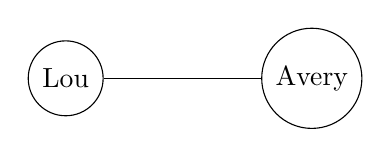
\begin{tikzpicture}
	\draw
	(1,1) node[anchor=east,circle,draw]{Lou}--
	(3,1) node[anchor=west,circle,draw]{Avery};
	\end{tikzpicture}
	\caption{The trivial graph underlying the one-shot Prisoner's Dilemma}
\end{figure}
Similarly, for the tournament if we call the players $p_1,...,p_n$, the tournament was a repeated game on a \textit{complete graph}. This is the graph with each vertex connected to everyother vertex: $K_n=\{\{p_1,...,p_n\},\{(p_i,p_j):\forall i\neq j\}\}$\\

\begin{figure}
	\centering
	\begin{subfigure}{.5\textwidth}
		\centering
		\includegraphics[width=.9\linewidth]{K5.pdf}
		\caption{$K_5$}
		\label{fig:K5}
	\end{subfigure}%
	\begin{subfigure}{.5\textwidth}
		\centering
		\includegraphics[width=.9\linewidth]{K16.pdf}
		\caption{$K_{16}$}
		\label{fig:K16}
	\end{subfigure}
	\caption{The Complete Graphs $K_5$ and $K_{16}$}
	\label{fig:complete graphs}
\end{figure}

\subsubsection{Some new Graphs}
Now we have made the graphs we are playing games on explicit we can try some new ones.\\
A graph often used in models is the 2D lattice as it is both instructive and relatively easy to analyse.\cite{eq_of_life}\\
\begin{figure}
	\centering
	\includegraphics[width=.5\linewidth]{2d_lattice.pdf}
	\caption{A 2D lattice}
\end{figure}
The von Neumann neighbourhood of the 2D lattice (Figure \ref{fig:vonneumann}) makes each point a neighbour of the $4$ points vertically and horizontally next to it.\\
\begin{figure}
	\centering
	\begin{subfigure}{.5\textwidth}
		\centering
		\includegraphics[width=.9\linewidth]{vonNeumannNeighbourhood.pdf}
		\caption{The von Neumann Neighbourhood}
		\label{fig:vonneumann}
	\end{subfigure}%
	\begin{subfigure}{.5\textwidth}
		\centering
		\includegraphics[width=.9\linewidth]{mooreNeighbourhood.png}
		\caption{The Moore neighbourhood}
		\label{fig:moore}
	\end{subfigure}
	\caption{Different neighbourhoods on the 2D Lattice}
	\label{fig: lattice neighbourhoods}
\end{figure}
The Moore neighbourhood of the 2D lattice (Figure \ref{fig:vonneumann}) includes the nearest vertical and horizontal neighbours as well as the nearest diagonal points.\\
To avoid boundary effects when playing games on these lattices (i.e. the side players having fewer opponents), we can 'wrap' the 2D lattice around itself to create a torus. So each neighbour at the top of the lattice is joined to the neighbour in the same column displayed visually at the bottom of the lattice.
\subsection{Prisoner's Dilemma on a Torus}
\subsubsection{Setup}
We can extend the Prisoner's Dilemma to a repeated game on  2D Lattice.\\
Initialisation:\\
Make an $n \times n$ grid with wrapped ends to avoid boundary effects, creating a torus. Then let each vertex be a player of the Prisoner's Dilemma. In the first round, each player plays $C$ with probability $p$ and $D$ with probability $(1-p)$. They play their strategy simultaneously against every player in their Moore neighbourhood (Figure \ref{fig:moore}), using the same strategy against each of them.\\
Every stage after:\\
After playing the previous round, each player looks at their neighbours scores. They then adopt the strategy of the highest scoring neighbour as their strategy for the next round. Again they play the same strategy against every player in their neighbourhood.
The payoff matrix retains characteristics of the original given Prisoner's Dilemma and is given by:\\
\setlength{\extrarowheight}{2pt}
\begin{tabular}{cc|c|c|}
	& \multicolumn{1}{c}{} & \multicolumn{2}{c}{Lou}\\
	& \multicolumn{1}{c}{} & \multicolumn{1}{c}{$C$}  & \multicolumn{1}{c}{$D$} \\\cline{3-4}
	\multirow{2}*{Avery}  & $C$ & $(1,1)$ & $(\epsilon,b)$ \\\cline{3-4}
	& $D$ & $(b,\epsilon)$ & $(0,0)$ \\\cline{3-4}
\end{tabular}
\\
\\
where $\epsilon<1<b$.
\\

\subsubsection{Example Runs}
In this section we use values of a $100\times100$ grid, $p=0.5$ and $\epsilon=0$. We can create a wide variety of dynamic behaviour, including chaos and bifurcations by adjusting the value of $b$.
\subsubsection{Qualitative Analysis}
For $b>1.\bar{6}$, the board eventually tends to an equilibrium with mostly defectors. Clearly the rewards of non-cooperation are too high to a sustain a more socially optimal situation.
\begin{figure}
	\centering
	\begin{subfigure}{.3\textwidth}
		\centering
		\includegraphics[width=.9\linewidth]{/mooreLattice/1b=17.png}
		\caption{Early}
		\label{fig:dir}
	\end{subfigure}%
	\begin{subfigure}{.3\textwidth}
		\centering
		\includegraphics[width=.9\linewidth]{/mooreLattice/2b=17.png}
		\caption{Developing}
		\label{fig:loop}
	\end{subfigure}
	\begin{subfigure}{.3\textwidth}
		\centering
		\includegraphics[width=.9\linewidth]{/mooreLattice/3b=17.png}
		\caption{Equilibrium}
		\label{fig:undirected}
	\end{subfigure}
	\caption{The simulation running with $b=1.7$}
	\label{fig:complete graphs}
\end{figure}
Similarly, for $b<1.6$, the simulation tends towards a static equilibrium of mainly cooperators.
\begin{figure}
	\centering
	\begin{subfigure}{.3\textwidth}
		\centering
		\includegraphics[width=.9\linewidth]{/mooreLattice/1b=15.png}
		\caption{Early}
		\label{fig:dir}
	\end{subfigure}%
	\begin{subfigure}{.3\textwidth}
		\centering
		\includegraphics[width=.9\linewidth]{/mooreLattice/2b=15.png}
		\caption{Developing}
		\label{fig:loop}
	\end{subfigure}
	\begin{subfigure}{.3\textwidth}
		\centering
		\includegraphics[width=.9\linewidth]{/mooreLattice/3b=15.png}
		\caption{Equilibrium}
		\label{fig:undirected}
	\end{subfigure}
	\caption{The simulation running with $b=1.5$}
	\label{fig:complete graphs}
\end{figure}
Between these two parameter regions, exists the third which exhibits the most interesting behaviour with dynamics between cooperation and defection.
\begin{figure}
	\centering
	\begin{subfigure}{.3\textwidth}
		\centering
		\includegraphics[width=.9\linewidth]{/mooreLattice/1b=163.png}
		\caption{Early}
		\label{fig:dir}
	\end{subfigure}%
	\begin{subfigure}{.3\textwidth}
		\centering
		\includegraphics[width=.9\linewidth]{/mooreLattice/2b=163.png}
		\caption{Developing}
		\label{fig:loop}
	\end{subfigure}
	\begin{subfigure}{.3\textwidth}
		\centering
		\includegraphics[width=.9\linewidth]{/mooreLattice/3b=163.png}
		\caption{Dynamic equilibrium}
		\label{fig:undirected}
	\end{subfigure}
	\caption{The simulation running with $b=1.63$}
	\label{fig:complete graphs}
\end{figure}
\subsubsection{Quantative Analysis}
looking at individual squares
%\subsubsection{Prisoner's Dilemma on a Scale Free Graph}


